\chapter{Editor}\label{sec:editor}
There are a~number of requirements on the editor functionality, namely that
\begin{itemize}
	\item the setting should be in 3D, visual, intuitive and efficient,
	\item the import and export format should be simple and human-readable,
	\item the code should be open-source,
	\item it should be cross-platform for all major operating systems and
	\item it should contain image capture functionality\ignore{ that should produce verisimilitudinous images, lmao}.
\end{itemize}

There are many frameworks that support 3D, the two main groups being user interface software (Qt, GTK+, Electron, etc.) and game engines (Unreal Engine, Godot, Source, Three.js, etc.).
The choice was made to use a~game engine because the main functionality of the editor is moving around and interacting with objects in 3D, which game engines are arguably more suited for.

Unity was chosen as the framework to implement the editor in, mainly due to the author's experience with Unity and C\# in general, along with a~large ecosystem of packages that were used to simplify the implementation and allow for rapid prototyping (see section \ref{sec:progdoc}).

The editor code is open-source and cross-platform (Linux, Windows, Mac), with newest releases being freely available at the \href{https://github.com/Climber-Tools/Cled/releases}{project releases page}.

\section{Functionality}

\subsection{Movement}
Movement is implemented using keyboard in a~way commonly used in 3D programs.
The arrow or \verb|WSAD| keys provide left, right, forward and backward movement, while the \verb|Space| and \verb|Shift| keys allow flying up and down.

Physics and gravity are also implemented, with the character being pulled to the ground when not flying, and colliding with both the wall and the holds.

\subsection{Wall and hold format}
For the editor to correctly load the scene, it expects the wall and holds to be in the Wavefront object (\verb|.obj|) file format, possibly with a Material Template Library (\verb|.mtl|) file and a~corresponding bitmap texture.
It has specific requirements on naming and location of the files, which differs slightly from Clis.
This is because the editor uses only a~subset of the files generated from Clis along with a~few that Clis doesn't generate.
To make things easier, the editor contains a~Python script to perform the import automatically.

The wall can also contain a~\verb|yaml| metadata file for wall-specific things: the possible route grades, names of the setters and wall zones.
This is to simplify editing route properties by selecting the right option from a~dropdown, instead of having to manually type it in.
Here is an example of one such file:

\begin{minted}{yaml}
Grades: ["black", "purple", "red", "salmon", "blue", "yellow"]
Setters: ["Danny", "Bert"]
Zones: ["pool", "overhang", "comp"]
\end{minted}

\subsection{Editor modes}
The editor contains three modes in which it operates, with the current mode being always displayed in the top right.
While this might seem like an implementation detail, it is helpful for general usage, because the user always knows which state the editor is in and can refer to the respective part of the documentation.
An obvious inspiration is the Vim text editor \cite{vim}, which uses the same concept.

The modes are the following:

\begin{itemize}
	\item \textbf{NORMAL} --- the mode the user is normally in; hovering highlights holds, which can be either picked up or selected
	\item \textbf{HOLDING} --- the mode in which the user is holding a~specific hold and can place it, or switch to the previous/next one from the selection
	\item \textbf{ROUTE} --- the mode in which the user is modifying the selected route by adding/removing new holds or modifying the route parameters
\end{itemize}

\subsection{Hold selection}
Quickly selecting which holds to place on the wall is crucial for effective virtual route setting, because it largely dictates the time the route setting takes.
The editor contains a~menu (accessed via pressing either \verb|Tab| or \verb|Q|) from which a~subset of holds can be filtered and used while editing.

Holds can be filtered by their color, type, manufacturer, or custom labels.
By default, the currently filtered holds are also sorted first by their color and then by their volume.
Additionally, hovering on each of the menu items rotates them around, which is useful when the static hold image isn't descriptive enough.

To make it further apparent which hold is currently held and which one is previous/next, all three are displayed at the bottom of the screen.

\begin{figure}[h]
	\centering
	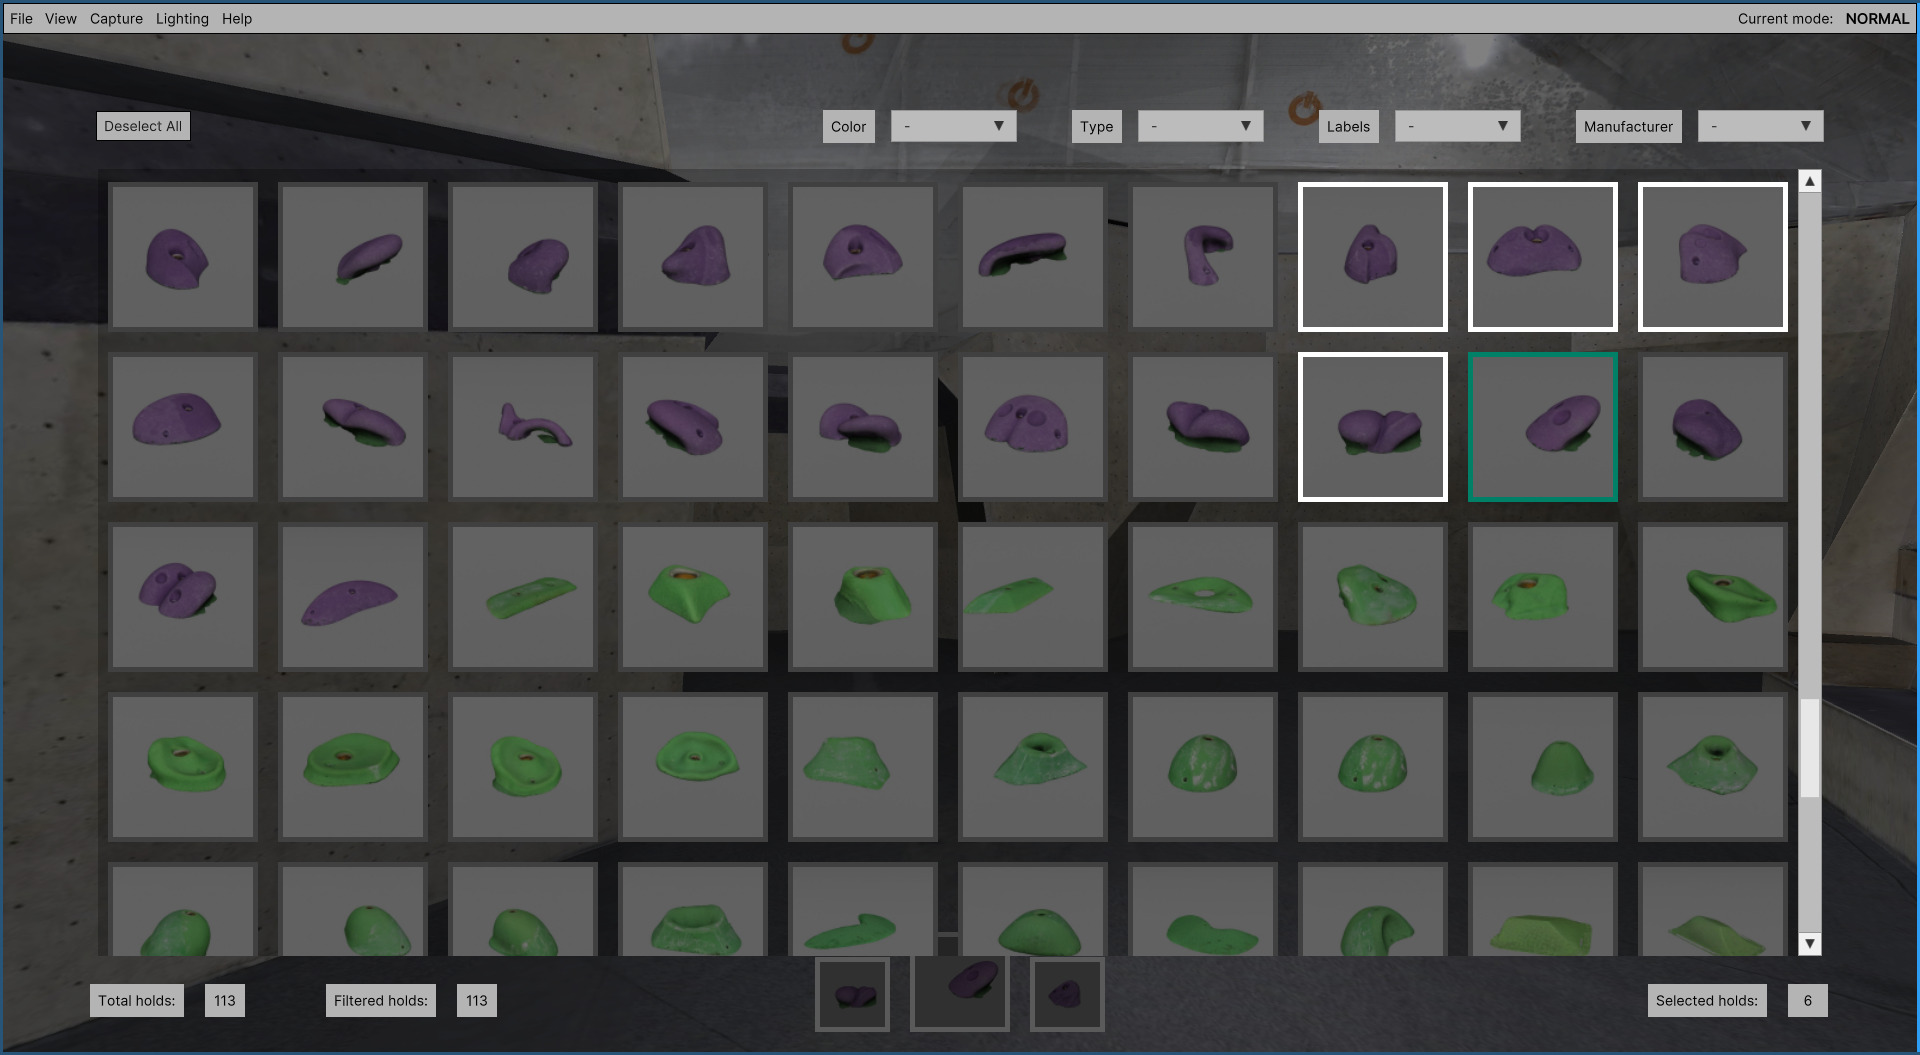
\includegraphics[width=\linewidth]{images/editor/picker.jpg}%
	\caption{The hold picker UI (no filters applied) on a~sample dataset.}%
	\label{fig:picker}
\end{figure}

\subsection{Import and Export}
The import and export format for the project files is a~human-readable \verb|yaml| file containing information about the state of the holds, routes, paths to the models and other metadata.
This makes usage in other applications easier (both for viewing and modification), since it is well readable and parseable.
Here is how the format looks like:

\newpage

\begin{minted}{yaml}
Version: 2.3.1 # Editor version (for compatibility reasons)

Player: # player settings
  Light: false # whether the player's light is on
  Position: # the player position as a vector
    x: 4.66010237
    y: 1.93126345
    z: -8.63198185
  Orientation: # the player orientation (up/down, left/right)
    x: 35.8053398
    y: 123.996086
  Flying: false # whether the player is currently flying

WallModelPath: /home/tom/Wall/wall.obj
HoldModelsPath: /home/tom/Holds

Holds: # a dictionary of hold instances
  f21cde933ad9: # a unique ID for the hold instance
    BlueprintId: 4bdff2704462 # an ID of the hold model
    State:
      Position: # the position of the hold in space
        x: 1.20504105
        y: 0.378549755
        z: -7.67928696
      Normal: # the normal of the hold, away from the wall
        x: 0.994500279
        y: 0.0156783238
        z: 0.103554823
      Rotation: 0 # the hold rotation about the normal
      Flipped: false # whether the hold is horizontally flipped
  0436ff53a1d8:
    BlueprintId: 4bdff2704462
    State:
      Position:
        x: 1.46525836
        y: 0.472094655
        z: -8.19389153
      Normal:
        x: 0.752805889
        y: -0.0226488542
        z: 0.657852829
      Rotation: 1.21387374
      Flipped: false

Routes: # a list of routes
- Name: The Nose
  Grade: VI
  Zone: El Capitan
  Setter: Mother Nature
  HoldIDs: # which hold instances the route contains
  - 0436ff53a1d8
  - f21cde933ad9

StartingHoldIDs: # a list of starting holds
- f21cde933ad9

EndingHoldIDs: # a list of ending holds
- 0436ff53a1d8

SelectedHoldBlueprintIDs: # a list of currently selected holds
- f21cde933ad9
- 0436ff53a1d8

Lights: # a list of point lights around the wall
  Positions:
  - x: 3.71035504
    y: 3.53241396
    z: -7.11679459
  - x: 5.59678602
    y: 3.53241396
    z: -3.97351503
  Intensity: 0.2 # how strong they are
  ShadowStrength: 0.2 # how hard their shadows are

CaptureSettings: # image capture settings
  ImagePath: /home/tom/Pictures # captured images path
  ImageSupersize: 2 # captured images resolution scaling
\end{minted}

\subsection{Building routes}
After holds have been placed, they can be combined to form routes by right-clicking to select a hold and then \verb|Ctrl| + left/right clicking to add other holds to the route.
Right-clicking an already selected route brings up the route settings menu (figure \ref{fig:routesettings}), from which various route attributes can be set.

\begin{figure}[t]
	\centering
	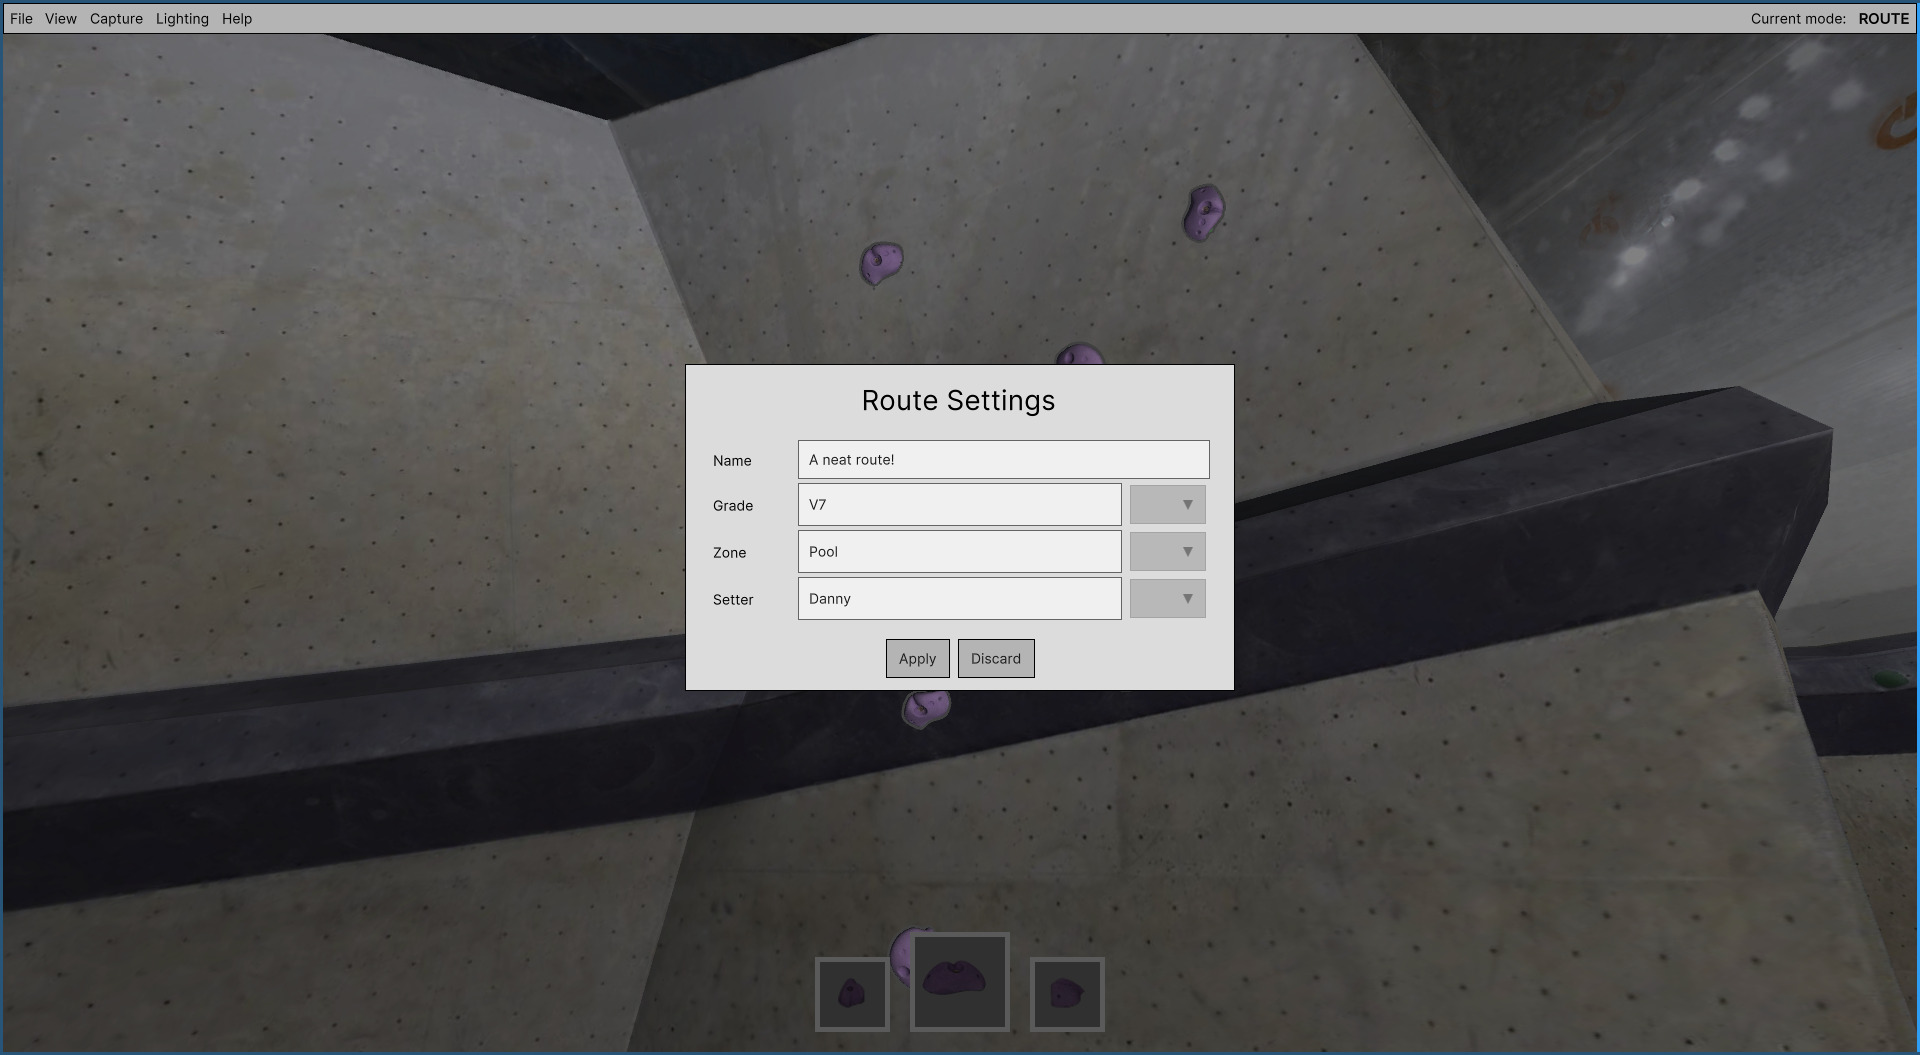
\includegraphics[width=\linewidth]{images/editor/settings.jpg}
	\caption{Route settings for a~sample route.}%
	\label{fig:routesettings}
\end{figure}

In addition, a~hold can be marked as the starting hold or the ending hold of a~route by hovering it and pressing \verb|t| (top) or \verb|b| (bottom) respectively.
The hold is then denoted by a~marker, as seen in figure \ref{ref:topbotmarkers}.
This marker always moves to the bottom of the hold so it is visible, no matter the hold position and orientation.

\begin{figure}[h]
	\centering
	\subfloat{{\includegraphics[height=3cm]{images/markers/1.jpg} }}%
	\hfill
	\subfloat{{\includegraphics[height=3cm]{images/markers/2.jpg} }}%
	\hfill
	\subfloat{{\includegraphics[height=3cm]{images/markers/3.jpg} }}%
	\hfill
	\subfloat{{\includegraphics[height=3cm]{images/markers/4.jpg} }}%
	\caption{Marker position on the same hold with different orientations.}%
	\label{ref:topbotmarkers}
\end{figure}

\subsection{Capturing images}
The editor contains functionality for capturing the current image of the wall.
This can be done anywhere in the editor by either selecting the option from the toolbar, or by pressing \verb|Ctrl+P| (see figure \ref{fig:capture}).
The image is then saved to the default system "Pictures" folder, unless configured otherwise.

\begin{figure}[h]
	\centering
	\subfloat{{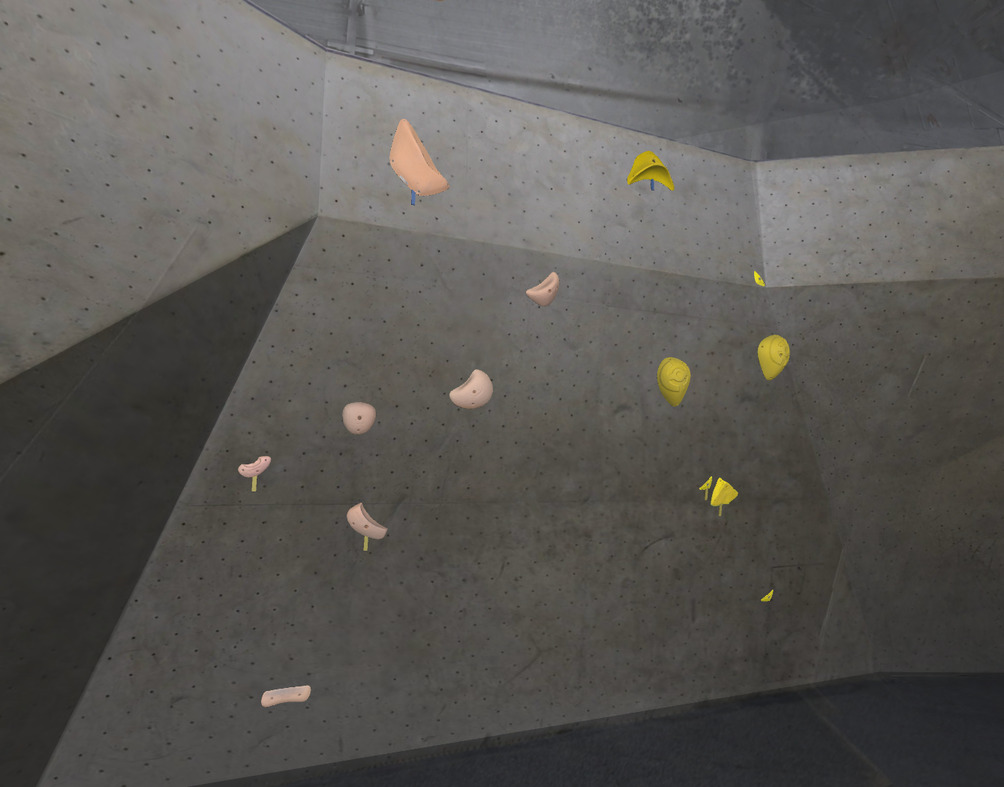
\includegraphics[height=5cm]{images/editor/capture-1.jpg} }}%
	\hfill
	\subfloat{{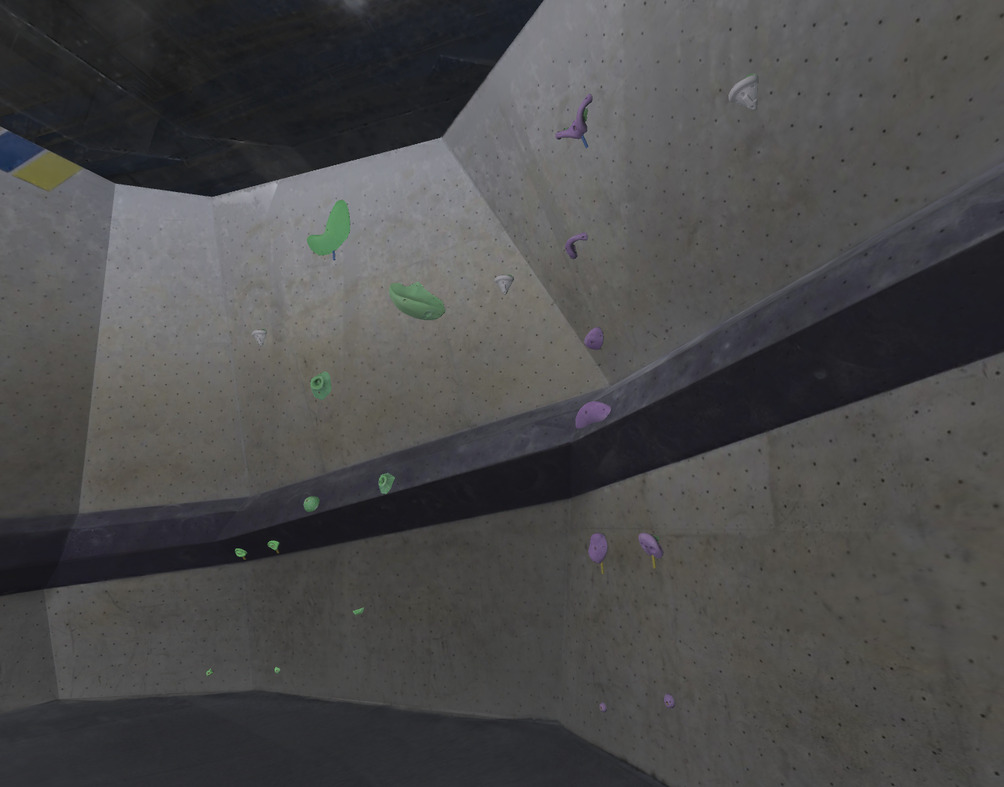
\includegraphics[height=5cm]{images/editor/capture-2.jpg} }}%
	\caption{Images generated using the editor capture functionality.}%
	\label{fig:capture}
\end{figure}

\subsection{Lighting}
Since each wall has different lighting needs and specifying them in the wall metadata would be too impractical, the editor supports placing lights on the current player position and removing them.
This can be done either from the \verb|Lighting| section of the toolbar, or by using \verb|F| to toggle the player lighting and \verb|Ctrl+F| to place one at the player position.

\section{Developer Documentation}\label{sec:progdoc}

The project has been developed on Linux in Unity Editor 2021.2.19f, using Rider as the code editor of choice.
All of the code (besides the freely used packages, which have their own licensing) is licensed under GPL-3.0, chosen for the perpetual availability of the source code for any and all derived works.

In addition to the editor code, the following free packages were used:

\begin{itemize}
	\item \textbf{Quick Outline} \cite{quickoutline} --- object outline creator,
	\item \textbf{Runtime OBJ Importer} \cite{objimport} --- an \verb|.obj| file importer and
	\item \textbf{Unity Standalone File Browser} \cite{unitystandalonefilebrowser} --- a~cross-platform file browser.
\end{itemize}

The new Unity UI package (UIElements) was used for creating the user interface.
It uses structured UXML (Unity XML) files to describe each respective UI part, which are styled using USS (Unity Style Sheets).
It was chosen over the older, GameObject-oriented approach because it is more structured and scalable (no need to manually create game objects).

Git is used for version control, with the entire repository being hosted on GitHub \cite{cled}.
Each release is automatically built for all supported platforms from the source code using GitHub Actions on tagged commits.
The version numbering scheme follows Semantic Versioning 2.0 \cite{semver}.

\subsection{Building from source}
To build the project from source, first clone the repository.
Next, open the project either by adding it to Unity Hub, or by using the Unity Editor 2021.2.19f (other 2021.x versions will likely also work but weren't tested).
Finally, build the project by pressing \verb|Ctrl+B|.

\subsection{Project structure}
The codebase can be broadly split into the following parts:

\begin{itemize}
	\item Controller classes:
	\begin{itemize}
		\item \verb|CameraController| --- controls the camera movement
		\item \verb|MovementController| --- controls the player movemen
		\item \verb|EditorController| --- controls interaction with holds
		\item \verb|UIKeyboardController| --- controls UI using the keyboard
	\end{itemize}
	\item Manager classes:
	\begin{itemize}
		\item \verb|EditorModeManager| --- manages the current editor mode
		\item \verb|HighlightManager| --- manages hold highlighting
		\item \verb|HoldStateManager| --- manages the state of the holds
		\item \verb|LightManager| --- manages the wall lights
		\item \verb|RouteManager| --- manages routes
		\item \verb|Preferences| --- manages preferences
	\end{itemize}
	\item User Interface classes:
	\begin{itemize}
		\item \verb|BottomBar| --- controls bottom bar
		\item \verb|HoldPickerMenu| --- controls hold picker menu
		\item \verb|LoadingScreenMenu| --- controls loading screen
		\item \verb|PauseMenu| --- controls the pausing
		\item \verb|PopupMenu| --- controls the popups
		\item \verb|RouteSettingsMenu| --- controls route settings menu
		\item \verb|RouteViewMenu| --- controls route view menu
		\item \verb|SettingsMenu| --- controls settings menu
		\item \verb|ToolbarMenu| --- controls the main toolbar
	\end{itemize}
	\item Import and Export classes:
	\begin{itemize}
		\item \verb|Importer| --- facilitates importing state
		\item \verb|Exporter| --- facilitates exporting state
		\item \verb|HoldLoader| --- loads the holds
		\item \verb|WallLoader| --- loads the wall
	\end{itemize}
	\item \verb|Utilities| --- random utility functions and classes
\end{itemize}

\subsection{Class interactions}

The interactions of the user with the code are done either through one of the controller classes (movement, camera, hold interactions) or through the UI classes (toolbar, hold picker, popups, etc.).

The manager classes encapsulate functionality that needs to be managed, such as the holds, routes, lights and highlighted objects.
They don't depend on any classes (the only exception being \verb|HighlightManager|, which relies on an instance of \verb|HoldStateManager| for making all holds transparent when a~route is selected).

The UI classes themselves have more complex dependencies due to the fact that certain parts of the UI depend on others. 
Examples include
\begin{itemize}
		\item \verb|BottomBar| displays the previous/current/next selected hold, which are stored in \verb|HoldPickerMenu|,
		\item \verb|RouteViewMenu| relies on \verb|SettingsMenu|, which it displays when one of its routes is double clicked and
		\item \verb|ToolbarMenu| contains buttons to display various other parts of the UI, such as \verb|SettingsMenu|, \verb|RouteViewMenu| and also \verb|HoldPickerMenu|.
\end{itemize}
